\documentclass[a4paper]{article}
\usepackage[utf8]{inputenc}
\usepackage[english]{babel}
\usepackage{biblatex}
\usepackage{lmodern,textcomp}
\usepackage{caption}
\usepackage{hyperref}
\usepackage{graphicx}
\usepackage{float}
\hypersetup{
    colorlinks,
%     citecolor=black,
    % filecolor=black
    linkcolor=blue,
%     urlcolor=black
}

\addbibresource{sample.bib}




\title{
Using Random Fourier Features with \\ Random Forests \\
\large Deliverable 6}
\author{Albert Ribes Marzá}

\begin{document}
    \maketitle
    \pagebreak

    \tableofcontents
    \pagebreak


    \section{Context and scope of the project}
        \subsection{Project formulation}

        Random Forest is a very powerful ensemble learning method than can be used both for classification and regression. It is based on building a group of Decision Trees (a forest) and output the prediction of the majority of them, and it corrects the problem of Decision Trees of over-fitting on the data\cite{RF}.

        The performance of this method can be very high, and it is a very commonly chosen methods for the following reasons\cite{RF-MIT}:

        \begin{itemize}
            \item It has a hight execution speed
            \item It doesn't over-fit on the data by increasing the amount of trees in the forest
            \item It can handle huge amounts of data
            \item It can achieve very hight accuracy
            \item It generates an estimate of the generalization error
        \end{itemize}

        However, in order to generalize on unseen data, the correlation between any two trees in the forest need to be very low. For this reason, it is needed a randomized sampling method to train each tree in a different way. At the same time, each of the trees should have a low error rate, so having a good sampling method is important.

        Many methods have been proposed, but most of them are based on hiding part of the data to the Decision Trees, and hence it affects on the performance of each individual one.

        I propose a different approach to lower the correlation among the trees in the forest. Instead of feeding them with the features of the original dataset, I suggest to map them to a randomized low-dimensional feature space, allowing the trees to use different mappings on the same data. This transformation is based on Random Fourier Features and it has been verified that it approximates various radial basis kernels\cite{RFF}.

        This approach has already been done with Deep Neural Networks\cite{RFF-NN} and has showed to be very effective, but it still haven't been studied on Random Forests. That's what I will study in this project.

        \subsection{Scope}

        The project will focus on training Random Forest with Random Fourier Features for classification problems.

        It will test the algorithm proposed against currently used Random Forests methods to see if it outperforms on accuracy or train time.

        To do so, the problem will first be addressed in the theoretical approach to find out the best way to mix those two techniques.

        Then, I will implement the ideas found in the first section in a programming language. I will use Python 3, since it is a powerful yet flexible language, suitable to work on machine learning and maths. In addition, it will allow me to use the \textit{scikit-learn} tools\cite{scikit-learn}, which contain a module with a Random Forest Classifier. It is a well tested library, and as it uses the 3-Clause BSD License, I will use the source code to build the Random Forest Classifier using Random Fourier Features, so I will not have to do it from scratch.

        Finally, I will test my implementation using public classification problem datasets, together with currently used Random Forest algorithms, in order to find the best tunning parameters and to see if it outperforms the state-of-the-art methods.

        \subsection{Possible obstacle and solutions}
            \subsubsection{Trouble in modifying the code}
            The plan is to modify the Random Forest Classifier implementation of the sklearn library to make it work as my algorithm describes. It is possible that it is so complicated to understand that I will not be able to modify it. If this is the case, I can use another equivalent implementation, for instance the one from R, which my project tutor happens to know, so I can receive help from him.

            If the problem persists, I will have to implement the code from scratch.

            \subsubsection{Computational power}
            The kind of problems the algorithm is expected to tackle are the ones with huge amounts of data to train. Although the training from this data is feasible for research groups with high computational power, I will only be able to use a laptop for the training. It may happen that I can not afford to commit the required time for training the data.

            If this happens, I will make the tests with tinier datasets and hope it to be representative to the real problems.

            \subsubsection{Find suitable public datasets}
            I plan to use public datasets to test my algorithm, but it may happen that I am not able to find a dataset with the required characteristics, such as type of problem, number of instances and attributes, etc.

            If this happens, I can create my own dataset with dummy data, as the aim of the project is not tied to a specific domain.


        \subsubsection{Methodology}
        During the realization of the project I will use the Waterfall Project Management methodology. The reason to chose that methodology is that the scope of the project is very well defined, and most of the tasks to do need to follow a sequential order. It is a simple methodology and it fits the requirements of this project.

        I will make a list of all the steps I need to accomplish the deliverable, assign a sequential sorting and decide when each particular task needs to be done. Then, I will start doing them one after the other.

        If it is possible, some of the tasks may overlap in time, as it may be useful to better match the different parts of the project.

        As the methodology is so simple, there are many tools and ways to follow it. The main tools I will use to follow it will be:
        \begin{itemize}
            \item \textbf{Trello}: a web based project management application to track the work to do, work in progress and work done.
            \item \textbf{Google Calendar}: To keep track of the deadlines and be notified on delivery days.
            \item \textbf{todo notes and todo notes trackers} such as todo-show from Atom text editor, to mark all the pending work.
        \end{itemize}

        \subsubsection{Development tools}
        The realization of the project will require the following development tools:

        \begin{itemize}
            \item \textbf{Git and Github}: used as a revision control system of the code and to the reports and securely store it in the cloud.
            \item \textbf{Python Programming Language}: all the code will be writen in this language
            \item \textbf{Python modules and libraries}: used for advanced maths and machine learning features, such as the Random Forest Classifier class from scykit-learn.
            \item \textbf{Text editor}: to write and modify the Python code
            \item \textbf{Testing datasets}: to evaluate the algorithm
            \item \textbf{A laptop}: for obvious reasons
        \end{itemize}

        \subsubsection{Validation methods}
        As each task will have a pre-fixed deadline, the validation method will consist of checking at a given date if I have finished all the things that needed to be done.

        Each week, at a definite day, I will check the list of things to do and the list of things done, and I will evaluate if the goals have been achieved.

    \section{Project planning}
    The estimated project duration is about 4 months. The project starts on Thursday \(1^{st}\) of February, 2018 and the deadline is on Monday \(18^{th}\) June, 2018.

    As a disclaimer, it must be pointed out that the initial planning could be revised and updated as a result of the evolution of the project.

        \subsection{Plan description}
        The whole project can be divided in 3 different sections. On the first one, Theoretical approach, I will focus on the study field in order to get a better understanding of the issues about mixing Random Forests with Random Fourier Features. On the second section, Algorithm Implementation, I will use the conclusions reached on the first one in order to implement the machine learning algorithm. Finally, in Testing, I will compare the performance of the current Random Forest algorithm with the implemented one, both in accuracy of results and in running time.

        It must be noted after the Testing section, depending on the results obtained, it is possible that a little bit more of work in the other sections may be needed, if there is a real believe that it can be improved with the extra effort. This work is not explained in the following sections, but it is planned to be done after the testing section.

        In addition, the composition of the final document for the project is an important part, but it is not included in the 3 sections described above.

            \subsubsection{Theoretical approach}
            This section doesn't require special tools to be achieved, but it can be divided in several subsections, apart from a general understanding of the fields of the project:

                \subsubsection*{What kernel function should I choose to approximate?}

                The Random Fourier Features extraction core idea is to produce a mapping of the original features of the data which is an approximation of a shift-invariant kernel function. This feature space is the one we are going to use to feed the Random Forest to build a good classifier.

                Hence, we have to decide what is a good kernel function to be approximated.

                \subsubsection*{What is the suitable dimensionality of the new feature space derived from the mapping?}

                The number of features in the new space doesn't need to be the same as in the original space. It can be much lower, which can be good to improve the training speed.

                It must be decided what is the best dimensionality to feed the Random Forest.

                \subsubsection*{What changes should be made to the original algorithm in order in order to correctly handle the new mapping of the features?}

                The original Random Forest Algorithm is not designed to be used the way we want, so we will have to decide what changes are needed to be made in order to get good results. Some of the decisions we will have to make will be: will we feed the trees in the forest with the same mappings, or with a random subset of it, or with different mappings on the same data?; or: will we need to change the splitting conditions of the nodes in the trees?


            \subsubsection{Algorithm implementation}
            The implementation of the algorithm will be made using the Python 3 programming language. To do so I will need a computer, the source code of the scikit-learn tools together with the documentation and some machine learning and maths modules from Python 3. Several things will have to be done:

                \subsubsection*{Implement the random mapping of the data using the Fourier Features algorithm}
                This is just a simple module to map the original feature space to the new one.

                \subsubsection*{Get familiar with Scikit Random Forest Classifier module}
                This is strictly not implementation, but it is needed to proceed with the modification. I need to know how is the architecture of the original module in order to write the modifications and join them with the rest of the code.

                \subsubsection*{Modify the Scikit module to work with the new features}
                Just as the title says. It is expected that most of the original code will be used and I will only need to modify a tiny fraction.

                \subsubsection*{Debug the code}
                It is very likely that I will find bugs is my code, so I will have to fix it. It may take up an important amount of the algorithm implementation.




            \subsubsection{Testing}
                \subsubsection*{Look up suitable testing datasets}
                A real problem dataset is preferred for this testing, specially a dataset which which has been previously used for algorithm testing purposes.

                The dataset should be for a classification problem, and it is important to have a big number of instances, since the algorithm is intended to work and very big problems.

                If it is not possible to find a suitable datasets, I can build it from dummy data.

                \subsubsection*{Preprocess the testing datasets if needed}
                If the dataset is not in good conditions (number of missing or unknown values, abnormal values, etc.) I will have to preprocess it in order to fit the needs of the algorithm.

                \subsubsection*{Carry out accuracy tests}
                Just as asserted. A suitable metric will be used depending on the found dataset and the kind of problem.

                \subsubsection*{Carry out timing tests}
                Forgetting about the accuracy obtained (but assuming it is not too bad), it will be evaluated the time needed to successfully train the model, just to see if it is faster than currently used algorithms.

                \subsubsection*{Study the results of the testing}
                The point of all the project is to check if the suggested method performs well on several problems, so the results of the test will be studied to give an answer to the project.


        \subsection{Estimated time}

        \begin{center}
        \begin{tabular}{|c|c|}

            \hline
            \textbf{Task} & \textbf{Estimated duration (h)} \\
            \hline \hline
            Background approximation & 50 \\
            Decide the kernel & 6 \\
            Decide dimensionality & 4 \\
            Decide the changes & 10 \\
            \hline
            \textbf{Total theoretical approach} & \multicolumn{1}{|r|}{\textbf{70}} \\
            \hline
            Implement Fourier Mapping & 10 \\
            Get familiar with the module & 20 \\
            Modify the module & 20 \\
            Debug de code & 15 \\
            \hline
            \textbf{Total implementation} & \multicolumn{1}{|r|}{\textbf{65}} \\
            \hline
            Find testing dataset & 5 \\
            Preprocessing & 20 \\
            Accuracy tests & 10 \\
            Time tests & 10 \\
            Study the results & 10 \\
            \hline
            \textbf{Total testing} & \multicolumn{1}{|r|}{\textbf{55}} \\
            \hline
            \textbf{Repeat parts after testing} & \multicolumn{1}{|r|}{\textbf{20}} \\
            \hline
            \textbf{Composition of the final document} & \multicolumn{1}{|r|}{\textbf{30}} \\
            \hline
            \hline
            \textbf{Total project} & \multicolumn{1}{|r|}{\textbf{240}} \\
            % \bottomrule
            \hline

        \end{tabular}
        \end{center}

        \subsection{Gantt chart}
        \begin{figure}[H]
        \centering
        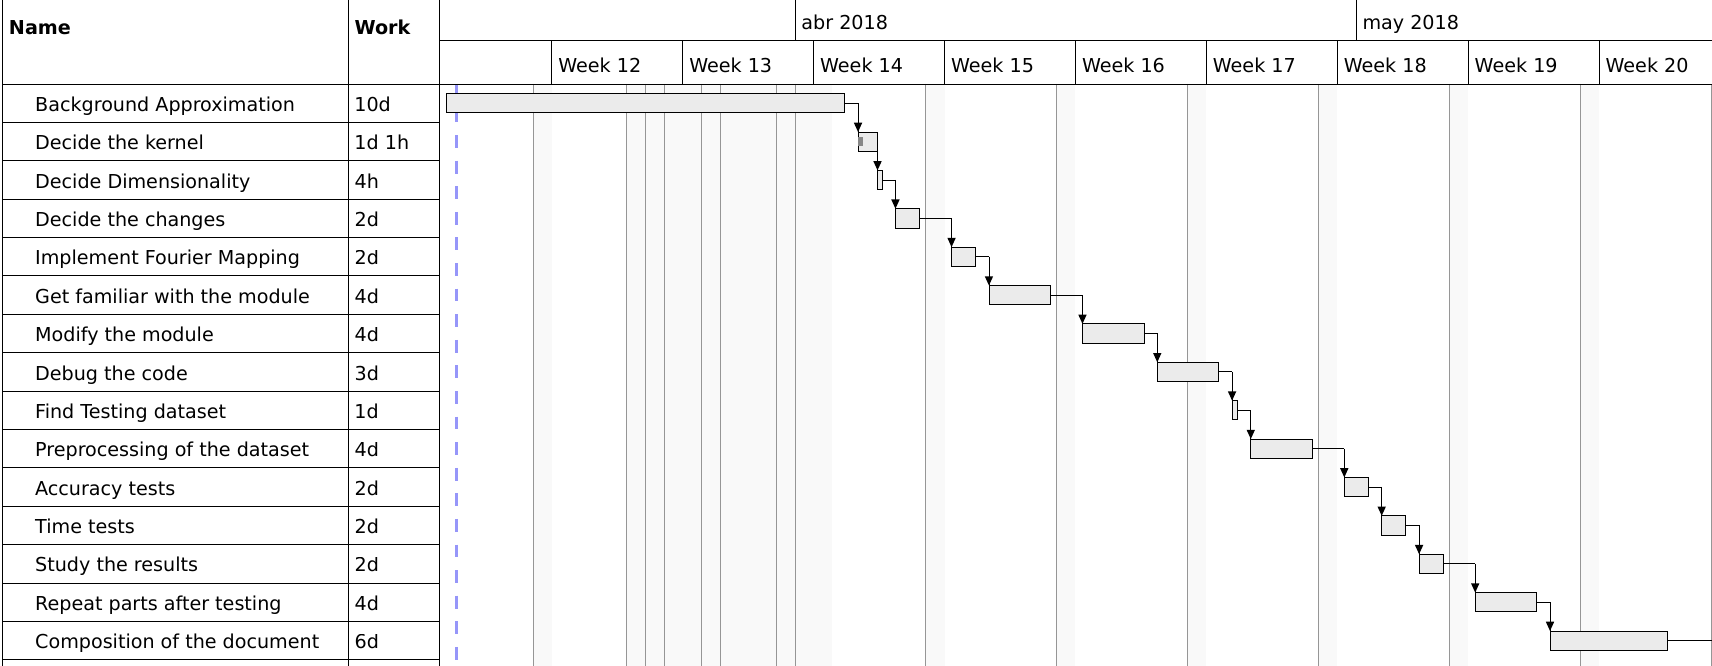
\includegraphics[width=\textwidth]{gant}
        \caption{Gantt chart of the whole project. The planning assumes 5 hours of work from Monday to Saturday and some rest during Holy Week}
        \end{figure}


        \begin{figure}[H]
        \centering
        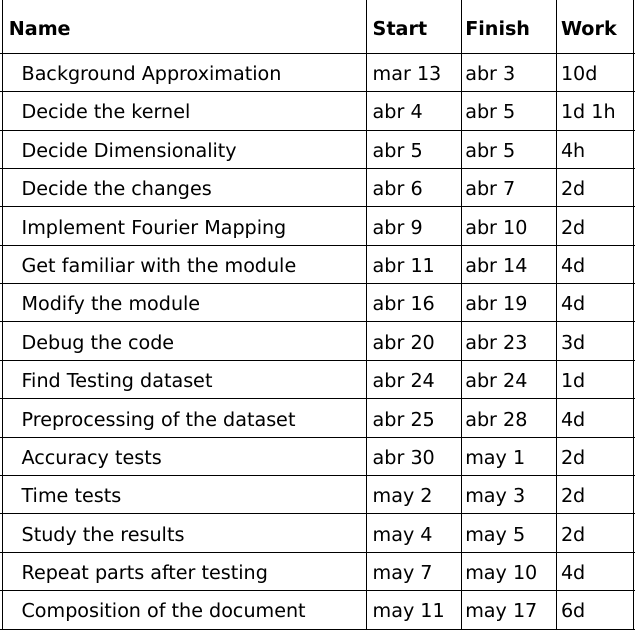
\includegraphics[width=\textwidth]{schedule}
        \caption{Schedule of the tasks}
        \end{figure}

        \subsection{Alternatives and action plan}
        As pointed out in the beggining of the document, the planning can be adapted from the initial one. As the Gantt chart shows, there are 4 weeks of margin from the scheduled end of the project and the deadline, so we have some flexibility. If a task task more than expected and there is not enough time, another task will have to be shortened.

        Here, some of the potential sources of delays are mentioned.

        \subsubsection{Complexity of the module}
        The Python 3 module from Scikit Project I plan to use may be too complicated to modify. I have planned much time in studying and modifying the code, but it could not be enough.

        \subsubsection{Bugs}
        I will certainly find bugs in my code. Detecting and correcting theme may be more laborious than expected, so it could delay the planning.



    \section{Budget and sustainability}
        \subsection{Environmental dimension}
            \subsubsection{PPP}
                During the production process of the project there will be needed power supply for charging the computer and general business resources such as light, heating, etc.

                The computer consumption is 10 W, and although it is not always the same, I will approximate the business resources as being 0.24kW, so the total consumption is 0.25 kW. As the project is planned to last 240 hours, the amount of power spent will be \(0.25 kW \times 240 h = 60 kWh\).

                The project doesn't generate residues.
            \subsubsection{Useful life}
                As this is project is a very theoretical study, it is hard to say what will be the environmental impact it will have during its useful life. If the conclusion of the project is satisfactory, it may help to develop more efficient machine learning algorithms which will need less energy spends and thus decrease the energy consumption.

            \subsubsection{Risks}
                The worst it could happen is that the conclusions reached with the project are useless and they do not help to improve efficiency in the machine learning algorithms.

        \subsection{Economic dimension}
            \subsubsection{Budget}
            \begin{table}
                \centering
                \begin{tabular}{|c|c|c|c|}
                    \hline
                    \textbf{Task} & \textbf{Time (h)} & \textbf{Money Spent (€)} \\
                    \hline
                    Backgroung Approximation & 50 & 1500 \\
                    \hline
                    Decide the kernel & 6 & 180 \\
                    \hline
                    Decide Dimensionality & 4 & 120 \\
                    \hline
                    Decide the changes & 10 & 300 \\
                    \hline
                    Implement Fourier mapping & 10 & 300 \\
                    \hline
                    Get familiar with the module & 20 & 600 \\
                    \hline
                    Modify the module & 20 & 600 \\
                    \hline
                    Debug the code & 15 & 450 \\
                    \hline
                    Find testing datasets & 5 & 150 \\
                    \hline
                    Accuracy tests & 10 & 300 \\
                    \hline
                    Time tests & 10 & 300 \\
                    \hline
                    Study the results & 10 & 300 \\
                    \hline
                    Repeat parts after testing & 20 & 600 \\
                    \hline
                    Composition of the document & 30 & 900 \\
                    \hline
                    \textbf{Total} & \textbf{240} & \textbf{7200} \\
                    \hline

                \end{tabular}
                \caption{It is considered a salary of 30 € / hour}
                \label{Tab:1}
            \end{table}


            \subsubsection*{Direct costs}

            All the software used in this project will be free, and thus they don't increase the cost of the project.

            The cost of the laptop will be specified in the ``Depreciation'' section.

            The workforce of the project consists of a single person working for 240 hours. Assuming a salary of 30 €/hour, the labour costs will be 240 hours \(\times\) 30€/hour = 7200€.

            Table \ref{Tab:1} shows the direct costs for each task in the project, and the costs of the whole project are summarized in table \ref{Tab:2}

            \subsubsection*{Indirect costs}

            As the workspace of the project will be the facilities of the FIB, transport service will be needed. I will use the public transport, so the cost will be 150 €.

            \subsubsection*{Depreciation}

            The cost of the computer needs to be depreciated. I expect it to have a lifetime of 7500 hours, and the project will spend 240, so the cost is a $3.2 \%$ of the total price of the computer. As it was 800 €, the cost of the project is $3.2 \% \times 800 = 25.6$ €.

            \subsubsection*{Unforeseen contingencies}

            The computer I plan to use to develop the project could have a breakdown. If this happens, the reparation or even replacement will increase the cost of the project.

            In order to avoid losing the work done, all the data will be securely stored in GitHub, where it is very unlikely to be lost.

            \begin{table}
                \centering
                % \label{}
                \begin{tabular}{|c|c|c|}
                    \hline
                    \textbf{Subject} & \textbf{Type} & \textbf{Amount (€)} \\
                    \hline
                    \hline
                    Workforce & Direct & 7200 \\
                    \hline
                    Transport & Indirect & 150 \\
                    \hline
                    Power & Fixed & Undefined$^*$ \\
                    \hline
                    Computer & Depreciation & 25.6 \\
                    \hline
                    \textbf{Total} & & 7375.6 \\
                    \hline
                \end{tabular}
                \caption{Total costs of the project}
                \label{Tab:2}
                $^*$ It is not possible to calculate that quantity since I will be using the facilities of the FIB
            \end{table}

            \subsubsection{Assessment}
            I expected that the costs for a project as ``simple'' as this one would be much fewer, since it involves very little extra costs apart from the salary of the worker. I find the cost is very high given the case that good results are not guaranteed, and I've learned that it is very important to first study the costs of a project, since the conclusions could not be intuitive.




        \subsection{Social dimension}
            \subsubsection{PPP}
                This project will teach me how to correctly plan and develop a good working methodology. As this is the fists big project I have to do, it will be very useful to see if only having good programming skills is enough to make projects get on. It will also teach me the easiest failure points in a big project, and will allow me to avoid them in more important projects in the future.

            \subsubsection{Useful life}
                Right now the algorithms used for training the Random Forest use some special kind of bagging which allows each node of the trees to use just a partition of the whole data. It is possible in this project that we find a better way to do the bagging allowing each node to see the entire dataset without loosing performance, or even improving it.

                It is possible that this project reaches satisfactory results, and it is possible that the method is proven not to be useful. In the first case it will help future studies to train a better learner, and in the second one, it will make other researchers know that this is not a good method, so they will not need to invest resources in performing the same study.

                Better learning algorithms are needed nowadays, so there exists a real need of this project and many others to try to develop them.

            \subsubsection{Risks}
                As the aim of this study is to provide knowledge, there are not real risks for this project. The worst it could happen is that the conclusions reached with the project are useless

    \section{References}











\printbibliography


\end{document}
